%!TEX root = ../thesis.tex
\chapter{Implementation}\label{implementation}

\ifpdf
    \graphicspath{{Chapter3/Figs/Raster/}{Chapter3/Figs/PDF/}{Chapter3/Figs/}}
\else
    \graphicspath{{Chapter3/Figs/Vector/}{Chapter3/Figs/}}
\fi

\NOTE{D}{General note: This book https://d2l.ai/index.html has good references for the original papers.}


\section{Two-Thinning}



\NOTE{A}{\textbf{Precondition at this point: I expect the reader to understand Deep Q-Learning well enough, so that I just have to note some implementation details. The same should be true about \TwoThinning. If anyone who reads this dissertation finds the explanation so far insufficient, let me know.}}


\subsection{Deep Q-Learning Implementation}


As there is no prior work on RL for the discussed balls-into-bins setting, I implemented the RL algorithms from scratch using PyTorch for the NNs. Even though there are some attempts at general purpose RL libraries (e.g.\ Stable Baselines ~\cite{hill2018stablebaselines}), they are very hard to customise at the moment. Following standard terminology, I will call the NN used by Deep Q-Learning as a Deep Q-Network (DQN). To discuss the implementation of Deep Q-Learning for \TwoThinning, I need the following definition.



\begin{definition} [slicing strategies]
Denoting the load vector at timestep $t$ as $v_t$, we call a \TwoThinning (or \KThinning in general) decision strategy \textit{\textbf{slicing}}, if it accepts a primary bin $i$ if and only if its load $v_t[i]$ is less than or equal to a \textit{\textbf{threshold}} $a$ (that can depend on $v_t$).
\end{definition}


There are two ways to formulate the \TwoThinning setting as a MDP. One is to treat (load vector, primary bin) pairs as states, and accept/reject as actions. The other is to treat load vectors as states, and thresholds for accepting/rejecting as actions. I chose the latter, because it implicitly restricts the search space to be explored by the RL agent to slicing strategies, which is justified by the following important (also intuitive) lemma:


\begin{lemma} \label{lemma: thresholdproperty}
There exists a slicing strategy that achieves the optimal expected final maximum load.
\end{lemma}


\begin{proof}
    \NOTE{A}{TODO}
\end{proof}

\NOTE{D}{Have you checked if there is a load vector, where it is better to use with probability $p_A$ threshold $f_a$ and with probability $1 - p_A$ threshold $f_b$? Andor: I don't understand. Take the one with a higher expectation, why would I use randomisation here?}


\subsubsection{Deep Q-Network (DQN)} \label{DQN}

The input to the DQN is a representation of the load vector $v$, and the output is an estimate of $Q(v, a)$ for each possible threshold $a$. We can observe the following constraints on the possible values of $a$:

\begin{itemize}
    \item It is enough to consider only integer thresholds, as the load values are integer too.
    \item It is always optimal to accept a bin with load $0$ (this is a corollary of Lemma ~\ref{lemma: thresholdproperty}), so $a\geq 0$.
    \item Thresholds $a$ larger than the maximum possible load $m$ have the same effect as using $a=m$.
    \item It is well-known that \OneChoice -- a less powerful protocol than \TwoThinning -- has a final maximum load less than $\Theta (\frac{m}{n} + \sqrt{\frac{m\log n}{n}})$ with high probability ~\cite{raab1998onechoice}. Therefore, we can further limit the search space by allowing only thresholds less than a chosen \textit{max threshold}. For the exact value of this hyperparameter and all the other hyperparameters explained later in this chapter (e.g.\ learning rate, hidden size of NN layers), see Appendix ~\ref{hyperparameters}. \NOTE{A}{This is important! If they miss it, I expect to lose around 20 marks. Any better place to put it but avoid the out of nowhere effect?}
    
\end{itemize}


Now, I will explain the input representation for the DQN. First of all, I always sort the load vector before feeding it into the network. This is possible because the order of the bins doesn't matter in \TwoThinning, unlike in \GraphicalTwoChoice. Sorting improves learning as the NN does not have to learn permutation invariance ~\cite{zaheer2017permutationinvariance}, and it will be important also for the actual NN architecture I use. Then, I one-hot encode each load value independently, because NNs often can't learn well with ordinal data. I use the natural $0$-$m$ range for one-hot encoding, but to reduce the number of weights of the NN I tried collapsing the very high load values (that have very small probability of occurring), into one ``outlier'' class, as shown in Figure ~\ref{NN-maxload}. This didn't provide better results, so I do not discuss it any further.


\begin{figure}[hbt!] \label{NN-maxload}
    \centering
    %\includesvg[scale=0.15]{Chapter2/Figs/NN_maxload.svg} -- it completely messes up the dots on the image
    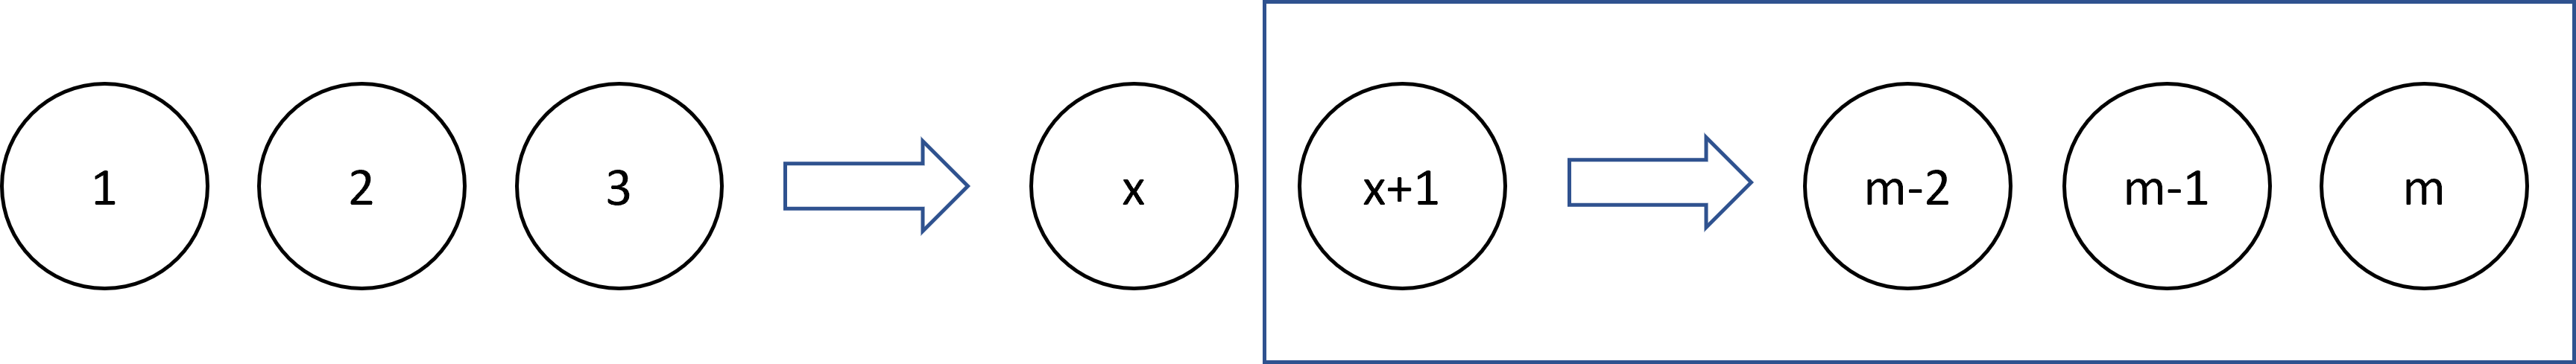
\includegraphics[scale=0.5]{Chapter2/Figs/NN_maxload.png}
    \caption{Potential grouping of (increasing) load values for one-hot encoding.}
\end{figure}


Now I turn to the discussion of the actual architecture of the DQN. Arguably, the highest loaded bins of a load vector are more important bins, since we care about minimising the maximum load.\NOTE{D}{Would be nice if you could support this in the evaluation. Andor: agree, it would be nice. Any specific ideas? Sounds difficult to analyse.} In the extreme, if the bin with the maximum load contained one more ball, that would be more significant than if an average loaded bin contained one more ball. Hence, my idea was to process the load vector in increasing order of the (one-hot encoded) loads, that is, in increasing order of importance. For this purpose, using a vanilla RNN -- which processes sequential data, inherently focusing more on later inputs -- is a perfect choice. I also tried the two more complex versions of RNNs (GRU, LSTM) mentioned in Section ~\ref{RNN}, but even though their desirable properties, they could not provide any improvement (partly due to the fixed-sized, relatively short input sequences \NOTE{A}{Should I be more confident or say that "probably" or "I hypothesise"?}), so I do not discuss them any further. \NOTE{D}{Would be good to refer to a figure in the evaluation section. Andor: yes, but there is no space to evaluate and compare exactly everything. Isn't it valid if I decide not to discuss it any further and focus on other things in the evaluation?}.
The hidden state of the RNN after the last input is fed through some number of fully convolutional (linear) layers to produce the estimates for $Q(v, a)$. As for the activation functions, I use ReLU for the linear layers, and $\tanh$ activation inside the RNN, following common practice (see e.g.\ ~\cite{szandala2020activationfunctions}).


\subsubsection{Stabilising Training}


In practice, Deep Q-Learning -- and in general any off-policy deep reinforcement learning algorithm -- can become unstable during training. There are several methods proposed in the literature to address this issue, and I implemented three of them that work well together in practice (see e.g.\ ~\cite{mnih2015dqnstabilitycombined}).


\paragraph{Experience Replay}
\NOTE{D}{Maybe start by what happens in your setting when you apply the vanilla Deep Q-Learning algorithm. And then mention how ``experience replay~~\cite{lin1992experiencereplay}'' solves this problem. }
\NOTE{D}{It might be helpful to split the paragraph into two: (i) what is experience delay and the problem it solves, (ii) how you implemented it}

Experience replay ~\cite{lin1992experiencereplay} is trying to solve the problem that in vanilla Deep Q-Learning, subsequent update steps are correlated -- e.g.\  in our case, after we update the weights of the DQN around a load vector with $x$ balls, we next update it around a load vector with $x+1$ balls. This correlation stems from updating in the same order as executing the actions in the game. In order to get the theoretical guarantees for these supervised learning-like updates, we need to have independent i.i.d. training samples. The idea in experience replay, is that instead of calling the update rule ~\ref{eq:deep-q-learning-update-with-semi-gradient} on the current $(s, a, s', r)$ tuple, we store this tuple in an experience replay buffer. Then, after every fixed number of steps, a batch of tuples are sampled uniformly at random from the buffer, and the DQN is updated according to those tuples. Another benefit of the idea is that samples can be reused multiple times, leading to a more efficient learning. Nevertheless, there should be a size limit on the buffer to get rid of outdated samples, which I implemented using a deque data structure with a limited memory capacity. Finally, note that sampling a batch of tuples rather than a single sample when updating has been shown to have a stabilising effect ~\cite{qian2020batchingsgd}.


\paragraph{Target Network}


The main difference between Q-Learning and Deep Q-Learning is that in the former, during one step we only update a single value in the Q-table, while in the latter, due to the function approximation, many neighbouring values are also affected. This becomes problematic, since looking at the update rule ~\ref{eq:deep-q-learning-update-with-semi-gradient} for Deep Q-Learning, to update around a Q-value $Q_{\mathbf{w_t}}(s_t, a_t)$, a neighbouring Q-value $Q_{\mathbf{w_t}}(s_{t+1}, a')$ is used. This can lead to a blow-up in the Q-values, intuitively, as a chain reaction. The idea with target networks ~\cite{argueta1992targetnetwork} is to have two copies of the same network architecture: one whose weights are updated by the update rule, and one that provides $Q_{\mathbf{w_t}}(s_{t+1}, a')$ of the ``target'' part $r_{t+1}+ \max_{a'} Q_{\mathbf{w'_t}}(s_{t+1}, a')$ of the rule. This weights $w'$ of the target network are updated to that of the main network periodically, every fixed number of training episodes. Another way to think about this is a way to achieve the stability of ~\ref{eq:deep-q-learning-update-with-semi-gradient}, while still using the full gradient descent update rule.


\paragraph{Using a better Optimiser}


Expanding on update rule ~\ref{eq:deep-q-learning-update-with-semi-gradient}, which updates the weights (based on the gradient) using simple Stochastic Gradient Descent (SGD), SGD could be replaced by any other (more complex) optimiser, such as ADAM ~\cite{kingma2015adamoptimiser}. Briefly, it additionally adjusts the step size based on moving averages and variances of the gradient. I also added gradient clipping \cite{mikolov2012gradientclippingoriginal}, a widely used extension in deep reinforcement learning, which doesn't allow absolute gradient values to exceed $1$, hence prevents exploding gradients and has been shown to also speed up training ~\cite{zhang2020gradientclippingaccelerate}.



\subsection{Ideas Implemented for Improvement} \label{improvementideas}


In this section I outline ideas independent of the DQN that I implemented to improve the performance of my RL algorithm. Some of these are well-known general ideas in RL, while others are specific to the \TwoThinning balls-into-bins setting.


\subsubsection{Reward Shaping} \label{rewardshaping}

As discussed in Section ~\ref{RLintro}, the most direct way to formulate the \TwoThinning setting as a MDP is to only give a reward (equal to minus the maximum load) after a final state, i.e.\ when all the balls have been allocated. The problem with this is that rewards are very sparse -- concretely, the agent only receives one reward per episode. It is problematic because until the final rewards propagate back to earlier states (that is, load vectors with fewer balls), the updates at earlier states are not justified -- they use a zero reward and a randomly initialised next state to update the current state. Hence, the idea is to inject additional rewards into the MDP, while maintaining correctness: the optimal policy for the new modified MDP has to be optimal for the original one as well, and hence for the \TwoThinning protocol too. There is a very interesting result proved in ~\cite{ng1999rewardshaping} about exactly what extra rewards can be used while maintaining the same optimal and near-optimal policies: the extra reward, when moving from state $s$ to state $s'$ using action $a$ has to be in the form $\Phi(s')-\Phi(s)$, i.e.\ the difference of the so-called potential functions $\Phi$ of the two states. Intuitively, the potential function should denote an estimate of how good a state is with respect to the original (in our case final) rewards. Now I present the candidate potential functions that I have created:

\begin{itemize}
    \item
    $\Phi_{max}(v)=\mathrm{maxload}(v)=- \max_{i \in [n]} v[i]$, which naturally extends the final reward. This means that the reward is $-1$ if the ball is allocated to a bin with maximum load, otherwise $0$.
    \item
    $\Phi_{std}(v)=-\mathrm{std}(v)$, where $std(v)$ is the standard deviation of the load vector. Compared to $\Phi_{max}$, it differentiates also between bins with non-maximum load.
    \item
    $\Phi_{exp}(v)=\sum_{i \in [n]} e^{\alpha \cdot  (v[i] - \mathrm{avg}(v))}$, with $\alpha>0$ a hyperparameter controlling the steepness of the function as shown for an individual load value in Figure \ref{exponential-potential-alpha} \NOTE{A}{Why is it ??}, is the so-called exponential potential, which has first been introduced as a useful tool in proving bounds for balls-into-bins settings ~\cite{ghosh1999exponentialpotential}. As a relevant example,\NOTE{D}{Mention that this is a smoother version of the first one. Andor: what do you mean? I don't get it.} if the exponential potential of a load vector $v$ is $O(n)$, it follows that $\mathrm{maxload}(v) < \mathrm{avg}(v)+O(\log(n))$.
\end{itemize}


\begin{figure}[hbt!] \label{exponential-potential-alpha}
    \centering
    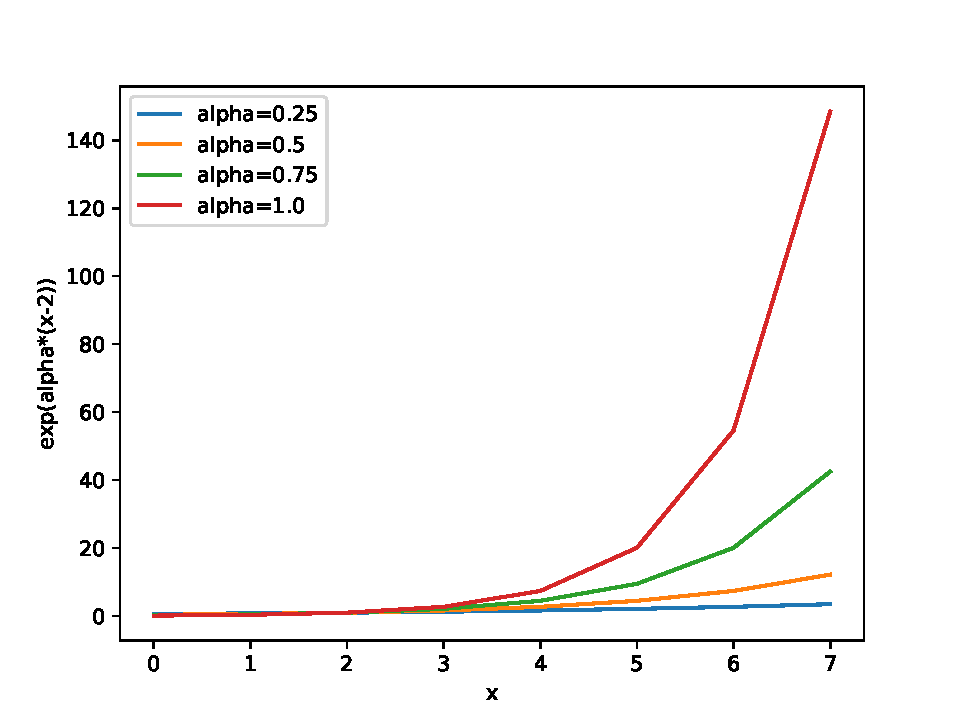
\includegraphics[scale=0.7]{Chapter3/Figs/exponential_potential_analysis.pdf}
    \caption{Showing the effect of different values of $\alpha$ to the exponential potential function with an average load of $2$.}
\end{figure}



\subsubsection{Curriculum Learning}


The idea of curriculum learning ~\cite{bengio2009curriculumoriginal} is to first provide easier problems to the agent, and just gradually increase the difficulty up to the original problem. I used this method as a pretraining phase for some number of \textit{pretrain episodes}. Without curriculum learning, the agent cannot learn as much as desired from the hard problems initially \NOTE{A}{Explain some more?}. For \TwoThinning, I implemented curriculum learning by first providing load vectors with $m-1$ balls allocated, then providing load vectors with $m-2$ balls allocated, and so on until starting from the original empty bins. To choose the training samples on level $k$ (i.e.\ where to place the initial balls), I had to choose load vectors with $m-k$ balls that are ``relevant'' -- there are exponentially many ways to place $m-k$ balls into $n$ bins, so it is not feasible to provide each of them to the agent. The heuristic I chose was to run the vanilla \OneChoice protocol with $m'=m-k$ balls, providing training samples distributed according to their occurrence when running \OneChoice, which is a closely related protocol to \TwoThinning. I decided to distribute the iterations between the levels according to an arithmetic progression, putting more weight on smaller $k$s.




\subsubsection{Normalised Load}

The notion of normalised loads mentioned in Section \ref{definitions} proved to be a very useful trick for RL training as well. Extending the notion to normalised thresholds (a normalised threshold $c$ at timestep $t$ is equivalent to a threshold $c+\frac{t}{n}$), we can consider slicing strategies with a constant \textit{normalised} threshold $c$. Unlike for constant \textit{unnormalised} thresholds, $c=0$ already gives a reasonable strategy (``mean thinning'') ~\cite{los2022cachingpackingthinningtwinning}, and learning a constant output is easy for a NN in the early episodes as well.


\subsection{Dynamic Programming}


For smaller values of $n$ and $m$ we can use dynamic programming based on the Bellman equation ~\ref{eq:bellmanState} to get the exact optimal policy. In general, dynamic programming approaches for RL problems are infeasible even for very small state spaces, but in this special case there are several insights that lead to a speed-up, and make it feasible for a broader set of $n$,$m$:


\begin{itemize}
    \item 
    As we did for the DQN, we can reduce the state space by\NOTE{D}{$\Theta(n!)$?} around a factor of $n!$, by treating permutations of a load vector the same state, i.e.\ using only sorted load vectors as states.
    \item
    While a general RL problem can contains\NOTE{D}{contain} cycles in the state transition graph (that is, the agent can possibly move around a loop), in this case it is a Directed Acyclic Graph (DAG) -- the next state always has exactly one more ball allocated. This is important, since we don't need to perform a fixed point iteration ~\cite{rhoades1991fixedpointiteration}, we can directly calculate the values based on a recurrence relation (see below).
    \item
    We can exploit Lemma ~\ref{lemma: thresholdproperty}: instead of using one dynamic programming state for each $Q(s,a)$ (storing a boolean value in each of them), we will have states of the form $V(s)$ (storing the optimal threshold in each of them). I also implemented a slower version of dynamic programming without using this lemma, on which interestingly I could test the validity of the lemma for specific values of $n$ and $m$.\NOTE{D}{Make a list of the observations/results you obtained}
\end{itemize}


Denoting $s[i]$ as the $i$th smallest load value in the load vector $s$, and $e_j$ as the corresponding unit vector $(0, 0, ... , 1, ..., 0, 0)$: \NOTE{T}{What is the range of $i$? Is it $i=1,2,\ldots,n$? But then you need to update the formula below.}

\NOTE{D}{For larger parentheses use $\left( \right)$}
\NOTE{D}{Use \begin{align}
    1 & = 2 + 3 \notag \\
    4 & = 5
\end{align}}
\begin{equation} \label{eq:twothinning-dynamicprogramming}
\begin{split}
    V_{\pi^*}(s) &= \max_a \mathbb{E} [r_{t+1} + V_{\pi^*}(s_{t+1}) \mid s_t=s, a_t=a] \\
    &= \max_{i \in [n]} \mathbb{E} [r_{t+1} + V_{\pi^*}(s_{t+1}) \mid s_t=s, a_t=s[i]] \\
    &= \max_{i \in [n]} (\sum_{0\leq j \leq i} \frac{1}{n}\cdot V_{\pi^*}(s+e_j) + \frac{n-i-1}{n} \cdot  \sum_{j \in [n]} \frac{1}{n}\cdot V_{\pi^*}(s+e_j))
\end{split}
\end{equation}
\NOTE{T}{can't we skip the first or second equation?}
where we used the fact that $r_{t+1}=0$ for non-final states, and that it suffices to use only thresholds that are equal to one of the load values. Since there are many possible final states, which serve as the base cases of the dynamic programming algorithm, it was more convenient to implement is using recursion and memoisation. The base cases are those load vectors $s$ that have all $m$ balls allocated, and for those we have $V_{\pi^*}(s)=-\mathrm{maxload}(s)$. \NOTE{A}{Exchange the last two sentences?}


We can observe that having already calculated $(\sum_{0\leq j \leq i} \frac{1}{n}\cdot V_{\pi^*}(s+e_j) + \frac{n-i-1}{n} \cdot  \sum_{j \in [n]} \frac{1}{n}\cdot V_{\pi^*}(s+e_j))$ for $i$, calculating it for $i+1$ takes $O(1)$ time,\NOTE{D}{Mention the speedup you get from this} since only a constant number of terms change, and the $\sum_{j \in [n]} \frac{1}{n}\cdot V_{\pi^*}(s+e_j)$ term can be pre-calculated upfront\NOTE{D}{When upfront?}. Hence, the overall runtime of the algorithm is $O(|states|\cdot n)$.\


Now I prove a small lemma limiting the possible improvements of an exact dynamic programming algorithm:


\begin{lemma} \label{lemma: everystatereachable}
For any load vector $v$ with $0\leq k\leq m$ balls in it, and any strategy, there is a non-zero probability of reaching $v$ during an execution.
\end{lemma}

\begin{proof}
    Simply observe that if the primary and secondary bins are the same, then whatever strategy is used, the ball will be allocated in that bin. Therefore, for any sequence of allocations there is a nonzero probability, and since any load vector can be reached by adding the balls one by one e.g.\ from left to right, all load vectors have a nonzero probability. \NOTE{A}{Isn't it too trivial? I mean it wasn't for me, but reading it now it seems trivial.}
\end{proof}
\NOTE{A}{A more interesting question is what would happen if we disallow the two choices to be the same. Then, there are several load vectors that the optimal policy can avoid, e.g.\ (0,0,0,0,m,0,0). How can we characterise these vectors?}
\NOTE{T}{I'm not sure you could reduce the space by that much. I think you can probably still get load vectors like (m/2,m/2,0,...,0).}

This means that all the possible states have to be taken into account when calculating the expectation.



Interestingly \NOTE{T}{I think this paragraph could be perhaps also dropped}\NOTE{D}{I think this is nice to have. You could also obtain some statistics like how many states have a high probability of being reachable or computing the entropy?}, there is no closed-form formula for the number of states, even for $m=n$ the number of states equal the so-called partition function $p(n)$ for which only approximate results are known: $p(n) \sim e^{\sqrt{n}}$ ~\cite{hardy1918partitionfunction}. I implemented the calculation of the number of states $f(m, n)$ as a function of $m$ and $n$, i.e.\ the number of increasing partitions of $m$ of size $n$, for which I also used dynamic programming:

\NOTE{D}{for $\to$ if?}
\NOTE{D}{comma after each case and full-stop in the last one.}
\begin{equation} \label{eq: numberofpartitions}
    f(m, n) = \begin{cases}
        1, & \text{for } m=0\\
        1, & \text{for } n=1\\
        f(m,n-1)+f(m-n,n), & \text{otherwise }
    \end{cases}
\end{equation}




\NOTE{D}{The values of $f$ confirmed the empirical performance of the DP algorithm.}The results from this secondary dynamic programming confirmed what I have seen about the efficiency of the main dynamic programming algorithm in practice. For example, for $n=10$, $m$ cannot exceed $60$, and for $n=30$, $m$ cannot exceed around $45$ so that it runs in time comparable to the training of Deep Q-Learning (few hours).\NOTE{D}{You will need to add a figure in the evaluation section.} These limits are indeed smaller than that of Deep Q-Learning, so while dynamic programming can provide the exactly optimal policy, it is not applicable for larger values. I note that the difference in the range of applicability of the two algorithms is perhaps surprisingly not very large\NOTE{D}{Are you sure?}. The main drawback of the dynamic programming algorithm is rather that it does not use function approximation, so it has to represent every state explicitly, which would cause memory error even before it would take too much time. \NOTE{A}{Add these rough estimates of n,m to Deep Q-Learning as well.}


\subsection{Other Strategies}

In addition to RL algorithms and dynamic programming, I implemented several other, more ``manual'' strategies. In Chapter ~\ref{evaluation}, these strategies will be compared against the strategies derived from the Deep Q-Learning training and dynamic programming.


\paragraph{Always Accept Strategy}
This is equivalent to \OneChoice, and it is included as a baseline. This is very robust, and requires no centralised information in a practical implementation.


\paragraph{Random Strategy}
This strategy accepts or rejects a ball\NOTE{T}{bin} with probability $p=\frac{1}{2}$. While I do not show it formally, it is easy to see that for the \TwoThinning setting this is equivalent to the Always Accept Strategy in performance. \NOTE{A}{Should I explain more?}

\paragraph{Mean Thinning Strategy}
This strategy always accepts a ball if it is below the current average load, and rejects otherwise. In a practical implementation, this would require only a centralised counter, and it has been shown that the performance doesn't decrease significantly if the counter is not exact ~\cite{los2022cachingpackingthinningtwinning}. 


\paragraph{Local Reward Optimiser Strategy}

While the goal of the agent in RL is the optimise the cumulative reward, a simplified goal can be optimising the immediate rewards. With rewards only after all the $m$ balls have been placed, this leads to all actions having an immediate reward of $0$, so for this strategy I will use the first reward shaping idea from Section ~\ref{rewardshaping}. This simplifies to getting a reward $-1$ if the balls gets allocated into one of the highest loaded bins, and a reward $0$ otherwise. Therefore, optimising immediate reward in this modified MDP leads to accepting any bin which is not a highest loaded one, and rejecting otherwise. Essentially, this strategy just tries to avoid increasing the maximum load in one step. It is easy to see that this is not an optimal strategy in general. \NOTE{A}{Give specific counterexample. I couldn't find any which is easy to see formally.}

\paragraph{The Threshold Strategy} 

This is a strategy that has been shown to be optimal \NOTE{T}{make clear that optimal means minimizing the gap at time $m$} ~\cite{feldheim2021thinning} up to a constant\NOTE{A}{I think multiplicative, but they probably won't care.}\NOTE{D}{Better to say multiplicative} factor for large $n$ and $m\leq O(n\cdot \sqrt{log(n)})$\NOTE{D}{$m = \mathcal{O}(n \cdot \sqrt(\log n))$}.\NOTE{T}{Minor: Use $\log n$ instead of $log n$.} This strategy accepts a bin, if and only if the primary allocations (i.e.\ number of times that bin has been chosen as the primary bin and the corresponding ball has been accepted) to that bin so far are less than a constant $l$. There are at least two surprising observations about this strategy. One is that it uses essentially a constant threshold, so it is not a very `adaptive'' strategy \NOTE{A}{Explain better}. Also, it is not hard to see that there should exist an optimal strategy whose decisions depend only on the current load vector, and doesn't take into account the past. On the other hand, this strategy differentiates between the same ball being allocated in the same bin as a result of a primary, or a secondary allocation. To the best of our knowledge, the reason for this reliance is to aid the proofs in the paper ~\cite{feldheim2021thinning}, and also it leads to an easily expressible strategy. 

\NOTE{D}{!!(So that I don't forget) The thinning upper bound in \url{https://projecteuclid.org/journalArticle/Download?urlId=10.1214\%2F21-ECP400} holds for any $n \geq 3$.}


\section{K-Thinning}


\subsection{Deep Q-Learning Implementation}


To frame the \KThinning problem as a MDP, I decided to use (load vector, number of choices left) pairs as states, and just like for \TwoThinning, thresholds as actions. The ``number of choices left'' part of the states indicate how many more bins can be rejected before the ball would be allocated into a randomly chosen bin. The state transitions happen according to the definition of \KThinning \NOTE{A}{Should I explain more?}. We still have the sparse rewards problem, so we need a suitable reward shaping function. I decided to use the same potential function as for \TwoThinning, that is I ignore the number of choices left for the potential function -- this way, I don't introduce any unnecessary bias, but still have less sparse rewards. 


For the neural network, I use a similar architecture as for \TwoThinning. The only difference is that now the input additionally contains the number of choices left. Keeping the RNN part applied on the load vector, I decided to bring in the number of choices left before the fully convolutional layers, by concatenating it with the final hidden state of the RNN. I applied one-hot encoding for the number of choices left as well, for similar reasons as for the load vector.


All the other parts of the implementation are analogous to the implementation for \TwoThinning (except for possibly different hyperparameters that I discuss later), so I omit those details from here. Same will apply for \GraphicalTwoChoice.



\subsection{Dynamic Programming}


A dynamic algorithm analogous to that for \TwoThinning has been implemented for \KThinning as well, with the states being (load vector, number of choices left) pairs.


The recurrence equations are: \NOTE{T}{What exactly is $v[i]$? Make notation consistent to 3.1 and 3.2}

\NOTE{D}{See comments above}
\begin{equation} \label{eq:kthinning-dynamicprogramming-0left}
\begin{split}
    V_{\pi^*}((v, 0)) &= \max_a \mathbb{E} [r_{t+1} + V_{\pi^*}(s_{t+1}) \mid s_t=(v,0), a_t=a] \\
    &= \max_{i \in [n]} \mathbb{E} [r_{t+1} + V_{\pi^*}(s_{t+1}) \mid s_t=(v,0), a_t=v[i]] \\
    &= \max_{i \in [n]} (\sum_{0\leq j \leq i} \frac{1}{n}\cdot V_{\pi^*}((v+e_j,k)) + \frac{n-i-1}{n} \cdot  \sum_{j \in [n]} \frac{1}{n}\cdot V_{\pi^*}((v+e_j,k)))
\end{split}
\end{equation}
\NOTE{D}{The extra line breaks that you have are increasing the white space (and you are loosing pages)}

and 
\NOTE{D}{Same here}

\begin{equation} \label{eq:kthinning-dynamicprogramming-xleft}
\begin{split}
    V_{\pi^*}((v, x+1)) &= \max_a \mathbb{E} [r_{t+1} + V_{\pi^*}(s_{t+1}) \mid s_t=(v,x+1), a_t=a] \\
    &= \max_{i \in [n]} \mathbb{E} [r_{t+1} + V_{\pi^*}(s_{t+1}) \mid s_t=(v, x+1), a_t=v[i]] \\
    &= \max_{i \in [n]} (\sum_{0\leq j \leq i} \frac{1}{n}\cdot V_{\pi^*}((v+e_j,k)) + \frac{n-i-1}{n} \cdot  V_{\pi^*}((v, x)))
\end{split}
\end{equation}

The runtime of this algorithm is $k$ times the runtime of the dynamic programming algorithm for \TwoThinning.


\subsection{Other Strategies}

Similar kind of strategies are possible for \KThinning as for \TwoThinning, with some adjustments.

\paragraph{Always Accept Strategy} Same as for \TwoThinning.


\paragraph{Random Strategy} In this case a number $x$ between $0$ and $k$ is sampled uniformly, and the $x$th choice will be the one accepted if $x<k$, and all the balls will be rejected if $x=k$.



\paragraph{Quantile Strategy} This strategy accepts a ball if there is less than $0.5$ probability of getting a better offer at later choices. To find this corresponding quantile with $x$ choices left, we solve the following equation for the quantile $y$:

\begin{equation} \label{meankthinning}
1 - (\frac{n-y}{n})^x = \frac{1}{2}
\end{equation}

which gives $y = n \cdot  (1 - 2^{-\frac{1}{x}})$, and then the threshold is $v[\floor{y}]$ where $v$ is the sorted load vector. \NOTE{A}{Explain better?}. Note that we could instead extend the Mean Thinning Strategy from \TwoThinning directly, but I do not consider that any further as that does not adapt to $k$.


\paragraph{Local Reward Optimiser Strategy} Choosing according to the expected immediate reward based on the reward function outlined above would lead to rejecting any bin with maximum load, and accepting otherwise.


\paragraph{The Threshold Strategy} This is a direct of extension of the analogous strategy for \TwoThinning: it accepts the $i$th choice if the number of times a ball has been allocated to the offered bin as an $i$th choice earlier is less than $l$. This strategy has been shown to be asymptotically optimal ~\cite{feldheim2020dthinning}.
\NOTE{D}{This is adaptive threshold, which changes for each load vector (so at every time step) and also depends on the sample number.}


\section{Graphical Two-Choice}



\subsection{Deep Q-Learning Implementation} \label{graphical-DQN}

To formulate this setting as a MDP, I use the most natural way: the states are (load vector, (bin1, bin2)) tuples, and the actions are booleans denoting which ball to choose. (Instead using load vectors simply as states would lead to a blow-up in the size of the action space, since we don't have any kind of threshold argument like for \TwoThinning). With the chosen formulation, it is very hard for the DQN, to learn a mapping with such an input shape, because bin1 and bin2 are indices (note that they cannot be just load values as that would ignore positional information) indexing the load vector, and indices are even worse for a NN than the simple ordinal data discussed for \TwoThinning \NOTE{A}{Add some reference?}. Therefore, I use the DQN to estimate the expected cumulative reward after allocating the current ball to bin1 or to bin2, and then I can greedily choose the bin with the higher such expectation. More formally, the input to the DQN is a load vector, and the output is a vector of the same shape, whose $i$th value denotes the expected cumulative reward if the next ball is allocated in bin $i$. \NOTE{A}{Is it clear?} \NOTE{A}{Is is a valid thing to do? I don't have a deep enough understanding...}


For the NN architecture, RNN is no longer a principled choice. The motivation for that in earlier settings was that it favours later inputs, and we can sort the load vector in increasing order, which also meant increasing order of importance. However, ordering the bins in this graphical setting would lead to destroying, and hence ignoring the connectivity information \NOTE{A}{Is it clear? I don't think so.}. Hence, I considered two options for the architecture. A simple fully convolutional (FC) network, which can possibly learn how to make use of the connectivity information, but there is no additional motivation for it to do so. Therefore, a more specialised architecture is any Graph Neural Network (GNN). GNNs are similar to Convolutional Neural Networks (CNNs) in that they also start by combining local information, and move towards the big picture. Due to length constraints on the dissertation, I don not consider GNNs any further, as I could get reasonable performance from a FC network as well. \NOTE{A}{TODO: Implement GNN and remove the last sentence.}



To tackle the sparse rewards problem, we could use any of the potential functions defined earlier. However, all of those functions ignore the graph structure, i.e.\ the edges. Intuitively, having many overloaded bins that are many hops away from each other is much better than having many overloaded bins close to each other, because if there are some underloaded bins next to an overloaded one, they can take away some of the future load from the overloaded bin. Therefore, motivated by this observation, I propose two new potential functions:


\begin{itemize}
    \item 
    $\Phi_{edge}(v)=\max_{x\sim y \in E} \min(v[x], v[y])$ \NOTE{A}{Why doesn't the argument go below the word "max"?}\NOTE{D}{Because it is inline. You can change to \[\Phi(v)=\max_{x\sim y \in E} \min(v[x], v[y])\]}, i.e.\ finding the worst edge, where no matter what strategy is used, an already highly loaded bin will be chosen.
    \item
    $\Phi_{neigh}(v)=\max_{x \in [n]} \frac{v[x]+\sum_{x\sim y \in E}v[y]}{deg(x)+1}$, i.e.\ finding the neighbourhood with the largest average. We will see this idea again in Section ~\ref{graphical-otherstrategies}.\NOTE{D}{Replace sentence with (see \cref{graphical-otherstrategies})}
\end{itemize}
\NOTE{T}{Maybe also add a list of the known potential functions?}

I provide a comparison of the various options in the hyperparameters section.


\subsection{Graph Structures}


Here I list the types of graphs on which I evaluate the algorithms. It is important that I train a separate RL agent for each graph, just like for each $n$, $m$ pair.


\paragraph{Complete Graph} This is exactly the \TwoChoice setting, for which Greedy is known to be the optimal strategy. This graph type serves as a baseline.


\paragraph{Cycle} The cycle graph with $n$ nodes numbered as $[n]$ has an edge between node $i$ and $(i+1)\%n$\NOTE{D}{$i+1 \pmod{n}$}. This is a very natural graph to investigate, since it comes up very often in computer systems, e.g.\ token rings.


\paragraph{Hypercube} The hypercube graph with $n=2^N$ nodes numbered as binary numbers in the range $[n]$ has an edge between two nodes iff there is exactly one bit difference between them. Hypercube graphs have several applications in network topologies ~\cite{ostrouchov1987hypercubenetwork} \NOTE{A}{Why? Why is it good?}.


\paragraph{Random Regular Graph} To better test the applicability of different algorithms, I create random regular graphs drawn (approximately) uniformly at random from all regular graphs with node $n$ of degree $d$. Interestingly, this is a challenging computational problem to do exactly uniformly at random -- even generating regular graphs is difficult. I applied the efficient randomised algorithm described as Algorithm 2 in ~\cite{steger1999randomregulargraphs}, and my code reliably generates regular graphs of size up to a few hundred with arbitrary degree.



\subsection{Dynamic Programming}


We can observe the same difficulties about \GraphicalTwoChoice for dynamic programming just like for RL. The main speedup for the dynamic programming algorithm for \TwoThinning was to look only at sorted loads. This is not possible here, as two bins with the same load are not interchangeable. Using load vectors as states, denoting by $G$ the graph, by $E$ its edges, and assuming that the nodes are numbered from $0$ to $n-1$, we get the following recurrence relation: \NOTE{T}{$x \sim y$ is enough, $x \sim y \in G$ looks a bit ood}


\begin{equation} \label{eq:graphicaltwochoice-dynamicprogramming}
    V_{\pi^*}(v) = \frac{\sum_{x\sim y \in G}\max_a (V_{\pi^*}(v+e_x), V_{\pi^*}(v+e_y))}{|E|}
\end{equation}


and we have $V_{\pi^*}(v)=-\mathrm{maxload}(v)$ for final states $v$.

This achieves an $O(|states|\cdot |E|)$ algorithm, and Lemma ~\ref{lemma: everystatereachable} gives confidence\NOTE{T}{Phrasing. ``confidence'', this sounds too vague. The lemma establishes or demonstrates?} that this is optimal for general graphs. Note that for the complete graph this is $O(n)$ times slower than the algorithm for \TwoThinning.

I will use this algorithm to construct a counterexample that Greedy is suboptimal. For that, I need to derive not only the values (as in the equation), but also the optimal decisions when faced with two bins. This is easily derivable from the memoisation dictionary. For the purposes of the counterexample, I distinguish not two, but three possible decisions: choose the first bin, choose the second bin, doesn't matter\NOTE{D}{informal}.


\subsection{Other Strategies} \label{graphical-otherstrategies}


\paragraph{Greedy Strategy} Choose the bin with the smaller load. If equal, choose uniformly at random.


\paragraph{Random Strategy} Choose uniformly at random between the two options.



\paragraph{Local Reward Optimiser Strategy} In this case, with the usual maximum load based potential function, this amounts to choosing the ball which is does not have maximum load, and choosing uniformly at random if they both or neither have maximum load.


\paragraph{Flow Based Strategy}

As I will explicitly show by generating a counterexample in Chapter ~\ref{evaluation}, Greedy is not optimal for \GraphicalTwoChoice -- the reason is that in this setting the bins are not independent, and their connectivity matters. The idea of the algorithm presented in ~\cite{bansal2021twochoicegraphical} is not to compare the load of the two offered bins, but compare the average load in a neighbourhood of the two bins (i.e.\ endpoints of the offered edge), taking into account topological information as well (note that this idea relates to my choice of potential function in Section ~\ref{graphical-DQN}). To achieve this, and crucially to find out which sets of bins to consider, their algorithm represents the preferences as a particular multi-commodity flow problem. It precomputes the sets of interests by solving the flow problem using an advanced data structure called R\"{a}cke-tree ~\cite{racke2008racketree}. During the actual allocation phase, the algorithm just compares the average load of two sets of size $O(log(n))$. I did not implement this algorithm due to its complexity (it could be a Part II project on its own), but it here as the best-known theoretical results for the \GraphicalTwoChoice setting -- it has been shown in ~\cite{bansal2021twochoicegraphical} to be optimal up to a polylogarithmic factor.


\NOTE{A}{Mention batched evaluation somewhere, and how I used GPU.}

\section{Hyperparameter Optimisation}

One of the biggest challenges of the project was to find the best set of hyperparameters, because there are many of them, so any kind of exhaustive search (e.g.\ grid search) is infeasible. Therefore I tried to use approximate hyperparameter search techniques, and combine them with expert knowledge to guide the search, and reduce the ranges. The expert knowledge mainly involves common values used in practice (e.g.\ learning rate), but involves domain-specific arguments as well (e.g.\ maximum threshold of DQN). In this section I describe the methods I used, and in Chapter ~\ref{evaluation} I analyse the results, and in particular the importance of each of the parameters. For the exact hyperparameter values I chose for the different settings see Appendix ~\ref{hyperparameters}.


\subsection{List of Hyperparameters}


First, I list the hyperparameters with some comments:

\NOTE{A}{Reorder in a more systematic way?}
\NOTE{A}{TODO: add usual values and/or reasons?}
\NOTE{A}{Should I add the ranges and options I used during the hyperparamter search?}
\begin{itemize} 
    \item batch size: the number of samples to take from the experience replay buffer using which the DQN is updated.
    
    \item $\epsilon$-start: for the $\epsilon$-greedy technique, it is common practice to gradually decrease $\epsilon$ during training. The reason is that after some training, less exploration is needed, as the best actions already start to take shape. I decrease $\epsilon$ according a negative exponential function, starting from $\epsilon$-start.
    
    \item $\epsilon$-decay: the decay parameter of the negative exponential function.\NOTE{T}{maybe better to use some formulas here?}
    
    \item $\epsilon$-end: as training goes on, $\epsilon$ converges to $\epsilon$-end.
     
    
    \item target update frequency: after every how many episodes is the target network synchronised with the main network.
    
    \item optimising frequency: this controls after every how many steps (i.e.\ actions) is the main network updated. Not updating it after every step is both a speed-up, and can control the reuse of samples in the experience replay buffer.
    
    \item memory capacity: the maximum size of the experience replay buffer.
    
    \item evaluation runs during training: to determine if the current model is better than the best one so far, I run this many full executions of the game with the current model, and average the scores. Note that this is very costly, as one execution of the game is equivalent to a full episode of training.
    
    \item maximum threshold of DQN: as mentioned in Section ~\ref{DQN}, the DQN is restricted to using only thresholds below this limit. A reasonable choice of this maximum threshold is around the target expected maximum load we expect to get, which can be estimated e.g.\ by the performance of simpler protocols, such as \OneChoice or \TwoChoice, or by theoretical results.
    
    \item loss function: the loss function to use between the current Q-value estimate and the new (``target'') Q-value estimate. \NOTE{A}{Explain better.}
    
    \item optimiser: the optimiser used for updating the neural network. \NOTE{A}{Update my code to include this as well.}
    
    \item learning rate: the learning rate of the optimiser. \NOTE{A}{Maybe I should also allow choosing other optimisers, such as simple SGD?}
    
    \item DQN -- hidden state size of RNN: this is the determines into how many numbers does the DQN have to ``compress'' the information about the load vector.
    
    \item DQN -- number of hidden layers of RNN: even though the main property of RNNs is that they process sequences, they can also have depth as well with any number of hidden layers.
    
    \item DQN -- number of linear layers after RNN: at least one layer is needed to bring the result to the right shape, but I allow more as well.
    
    \item potential function: some of the potential functions are only applicable to certain settings (e.g.\ \GraphicalTwoChoice).
    
    \item number of curriculum learning episodes: using curriculum as pretraining, this hyperparameter determines the overall number of episodes in pretraining.
    
    \item using normalised domain: this is a boolean choosing between normalised and absolute domain.
    
    


\end{itemize}


Note that the number of training episodes and the patience interval used for early stopping are not included in the hyperparameter search explicitly. This is because there isn't an optimal value for them based only on the score, as the score only improves by adding more episodes and not stopping early, it just takes more time. Therefore, I have run a first phase of the hyperparameter optimisation finding a sweetspot for the number of episodes, where the difference between the strength of different hyperparameters is already apparent (though the score could potentially improve by training longer), but it is still feasible to do several runs in a few hours. Then, during the main optimisation phase outlined below I have used a fixed number of episodes, and I didn't use early stopping \NOTE{A}{Should I explain why not?}.



\subsection{Hyperparameter Optimisation Methods}

Due to the difficulties of the large search space, I tried several methods for optimising the hyperparameters. One which is worth mentioning is a genetic hyperparameter optimisation algorithm ~\cite{wicaksono2018genetichyper}. The idea of genetic algorithms is to mutate hyperparameter combinations similar to human evolution, hopefully leading to a good combination after some generations.


Instead of genetic algorithms, I chose as my final choice Bayesian hyperparameter optimisation ~\cite{eggensperger2013bayesianhyper}. Just like genetic algorithms, this also tries to choose the next combination of hyperparameters to try more cleverly than simple grid search and random search, but in a more principled way. The idea is to train a secondary, so-called ``surrogate'' model, using Bayesian techniques based on the results for previous hyperparameter combinations. The motivation is that calling the actual model is very costly, but calling, and hence optimising the surrogate model is much cheaper, and hopefully still guides towards good hyperparamters for the original model.


I found the amazing Weights and Biases (WANDB) online tool ~\cite{biewald2020wandb} which is not just a framework for grid, random and Bayesian search, but also provides very useful insights e.g.\ into parameter importance, and automatically creates several analyses plots. The tool can be used by declaring the set of hyperparameters, connecting to the online server, choosing the optimisation method (and its parameters, e.g.\ I have set the number of rounds to $200$), and then reporting the scores from each run of the model to optimise.


Overall, I used the WANDB tool with the Bayesian option. Also, even though automatically tries to converge in the direction of good set of hyperparameters, it is just an approximation (and due to the large state space it is not very accurate), so I applied an iterative approach by running the Bayesian hyperparameter search with more and more refined ranges/options for the hyperparameters, based on previous iterations.


The optimal hyperparameters can differ between different settings, and between different values of $n$ and $m$. Therefore I have run different hyperparameter optimisation instances for each of the three different settings, and a representative subset of their subsettings, modifying $n$, $m$, $k$ for \KThinning and the graph for \GraphicalTwoChoice. I discuss the choices in more detail in Chapter ~\ref{evaluation}.


\section{Repository Overview}

\NOTE{T}{Is this section really needed? And the figure later? I would think some figures on RL learning or balls-into-bins might help the reader more}
The structure of the code repository is shown below. Only the most relevant files/folders are included here, and I do not expand two folders if they have a very similar substructure (e.g.\ $k\_thinning$ and $two\_thinning$). Note that there are multiple layers of evaluation: one next to the training files which were used mainly during implementation, one evaluation environment for each setting, which were used for analysing strategies in a principled way, and there is an evaluation folder which contains driver code and hyperparameter analysis.


\NOTE{A}{Should I add more files? e.g.\ non-deep RL attempts.}

{
\definecolor{folderbg}{RGB}{124,166,198}
\definecolor{folderborder}{RGB}{110,144,169}
\newlength\Size
\setlength\Size{4pt}
\tikzset{%
  folder/.pic={%
    \filldraw [draw=folderborder, top color=folderbg!50, bottom color=folderbg] (-1.05*\Size,0.2\Size+5pt) rectangle ++(.75*\Size,-0.2\Size-5pt);
    \filldraw [draw=folderborder, top color=folderbg!50, bottom color=folderbg] (-1.15*\Size,-\Size) rectangle (1.15*\Size,\Size);
  },
  file/.pic={%
    \filldraw [draw=folderborder, top color=folderbg!5, bottom color=folderbg!10] (-\Size,.4*\Size+5pt) coordinate (a) |- (\Size,-1.2*\Size) coordinate (b) -- ++(0,1.6*\Size) coordinate (c) -- ++(-5pt,5pt) coordinate (d) -- cycle (d) |- (c) ;
  },
}
\forestset{%
  declare autowrapped toks={pic me}{},
  pic dir tree/.style={%
    for tree={%
      folder,
      font=\ttfamily,
      grow'=0,
    },
    before typesetting nodes={%
      for tree={%
        edge label+/.option={pic me},
      },
    },
  },
  pic me set/.code n args=2{%
    \forestset{%
      #1/.style={%
        inner xsep=2\Size,
        pic me={pic {#2}},
      }
    }
  },
  pic me set={directory}{folder},
  pic me set={file}{file},
}

\begin{forest}
  pic dir tree,
  where level=0{}{% folder icons by default; override using file for file icons
    directory,
  },
[Project
    [helper, label=right:(useful reused helper functions and objects)]
    [two\_thinning
        [full\_knowledge
            [RL
                [DQN
                    [constants.py, file]
                    [neural\_network.py, file]
                    [train.py, file]
                    [evaluate.py, file]
                    [saved\_models, label=right:(I store here the best trained models for each $n$ and $m$)]
                    [curriculum\_learning]
                    [normalised\_load]
                    [...]
                ]
                [DeepSarsaRL]
                [PolicyGradient]
            ]
            [dp.py, file]
        ]
        [constant\_threshold]
        [average\_threshold, label=right:(only the average load is known to the agent)]
        [strategies, label=right:(strategy classes)
            [strategy\_base.py, label=right:(abstract base class), file]
            [mean\_thinning\_strategy.py, file]
            [...]
        ]
        [environment.py, label=right:(environment for analysing strategies), file]
        [...]
    ]
    [k\_thinning]
]
\end{forest}


(continued on the next page...)

\begin{forest}
  pic dir tree,
  where level=0{}{% folder icons by default; override using file for file icons
    directory,
  },
[Project
    [k\_choice
        [simulation.py, label=right:(code for running simple \OneChoice and \TwoChoice), file]
        [graphical
            [two\_choice
                [full\_knowledge, label=right:(as for \TwoThinning)]
                [graphs, label=right:(graph structures as classes)
                    [graph\_base.py, label=right:(abstract base class), file]
                    [cycle.py, file]
                    [...]
                ]
                [strategies, label=right:(as for \TwoThinning)]
                [environment.py, file]
            ]
        ]
    ]
    [evaluation
        [hyperparameter\_tuning]
        [analyses, label=right:(evaluation code and results)]
        [...]
    ]
    [unit\_testing]
    [dissertation]
    [proposal]
    [progress\_report]
]
\end{forest}
}


\NOTE{A}{Should I emphasize the OOP style more?}
\NOTE{D}{You should mention it somewhere. }
